%Plantilla para informes desarrollados para la Universidad Tecnológica Nacional Regional San Francisco, para la carrera de Ingeniería Electrónica.

\documentclass[12pt,a4paper,twoside,fleqn]{article}
\usepackage{graphicx} % Required for inserting images
	\graphicspath{{./img}}
\usepackage{fancyhdr} % Requeried for header and footer
\usepackage{makecell} % Requeried for header image
\usepackage{indentfirst}
\usepackage[spanish]{babel} % Paquete de idioma
\usepackage[font=footnotesize]{caption}
\usepackage{subcaption}
	
\usepackage{hyperref} % Genera vínculos en referencias y citas 
\usepackage{amsmath}
\usepackage{siunitx}
	\sisetup{
		group-digits=false,
		output-complex-root=j
	}

\usepackage{titlesec}

\DeclareCaptionFormat{label}{\fontsize{10}{10}\selectfont#1#2#3}

%\titleformat{\Comando de Estructura}[Tipo]{Formato}{Etiqueta}{Separación}{Código anterior}[Código posterior]

\titleformat{\section}[hang]
{\fontsize{14}{14}\bfseries}{\thesection.}{0.1cm}
{}

\titleformat{\subsection}[hang]
{\fontsize{12}{12}\bfseries}{\thesubsection.}{0.1cm}
{}
    
\begin{document}
\renewcommand\refname {}
\renewcommand\headrulewidth{0pt} % no line between document and header
\fancyhead{} % clear header
\fancyfoot{} % clear footer
\pagestyle{fancy}
\setlength{\headheight}{24.0pt}

\fancyhead[L]{\footnotesize
\mbox{\makecell[cl]{\includegraphics[height=20pt]{UTN_logo.jpg}}}
\makecell[cl]{Universidad Tecnológica Nacional \\ 15 Noviembre Año 2024 %fecha 
}}

\fancyhead[R]{\footnotesize
\makecell[cr]{Trabajo Integrador $4^{\text{to}}$ año\\ Ing. Electrónica}}

\fancyfoot[L]{\thepage}

\vspace{\fill}
{\huge \noindent \textbf{Medición de colores por reflexión utilizando resistencias dependientes de la luz (LDR)}} % title 
\vspace{1.5cm}
\par
\noindent
\textbf{Beck, Federico (autor)}\\
Departamento de Ingeniería Electrónica,\\ Facultad Regional San Francisco, Córdoba, Argentina.\\
\href{mailto:federicobeck91@gmail.com}{federicobeck91@gmail.com}\par
\vspace{0.5cm}
\noindent
\textbf{Perez, Mariano (autor)}\\
Departamento de Ingeniería Electrónica,\\ Facultad Regional San Francisco, Córdoba, Argentina.\\
\href{mailto:perezmariano7401@gmail.com}{perezmariano7401@gmail.com}\par

\section*{RESUMEN}
Un sensor de colores por reflexión permite determinar con precisión el color de un objeto al iluminarlo con una fuente de luz y midiendo la luz reflejada en el mismo. Un sensor típico emite luz blanca hacia un objeto, y mide la reflexión de cada componente de la luz blanca utilizando un arreglo de fotodiodos con filtros RGB. 

El objetivo de este trabajo consiste en desarrollar un dispositivo que permita determinar el color de un objeto mediante la técnica de reflexión, pero utilizando resistencias dependientes de la luz (LDR) sin filtros de color. Para ello se utilizará un LED RGB y se medirá la reflexión para cada color por separado.
\par
\noindent\textbf{Palabras claves:} Medición, color, reflexión, LDR, RGB.

\section*{INTRODUCCIÓN}
El color es una percepción visual que surge debido a la detección de diferentes longitudes de onda que no son absorbidas por un objeto o superficie. El conjunto de señales de distintas frecuencias compone el color de dicho objeto. Éstas, dentro del espectro visible de la luz, abarcan una gama de colores que va desde el rojo, con frecuencias más bajas y longitudes de onda más largas, hasta el violeta, con frecuencias más altas y longitudes de onda más cortas.\cite{ARPN_RGB_COLOR_SENSING}

Uno de los métodos para medir el color es mediante un dispositivo de detección especializado. En este proyecto, se ha desarrollado dicho dispositivo junto con su procesamiento digital correspondiente.

%explicar primero como funciona un LDR
El sensor consta de dos etapas, la primera esta compuesta por el emisor, el detector y su circuito de acondicionamiento. El emisor es un LED RGB capaz de emitir luz roja, verde y azul por separado, la cual será reflejada sobre el objeto a medir e incidirá sobre el detector. El detector utilizado es una resistencia dependiente de la luz, la cual varía su resistencia dependiendo de la luz que incide sobre la misma. La variación de resistencia se debe convertir en una variación de tensión para que pueda ser procesada, para ello se utiliza una fuente de corriente constante. Luego, la caída de tensión en los terminales del LDR se inyecta en un amplificador de instrumentación con ganancia unitaria, el cual cuenta con un alto rechazo al modo común y entrega en su salida una tensión igual a la diferencia de tensión en el LDR, que será procesada por la segunda etapa.

La segunda etapa abarca la recolección de datos y su posterior procesamiento. Mediante el conversor analógico-digital (ADC) se toman muestras de la salida del amplificador de instrumentación cuando la superficie a medir se ilumina con los distintos colores del LED RGB. Las muestras recolectadas posteriormente se pasarán por un filtro digital, el cual permitirá eliminar el ruido de linea y estabilizar las muestras obtenidas por el ADC. Finalmente, los valores de tensión muestreados y filtrados se convierten en un valor entero de 8 bits, que representará la intensidad de luz reflejada de la componente roja, verde, o azul. Una vez que se obtienen los valores de 8 bits para los tres colores se muestra el resultado medido en una página web.

Cabe recalcar que todas las mediciones se deben realizar aisladas de la luz ambiente, esto se logra mediante una carcasa impresa en 3D 
% la referencia a la figura podemos dejarla para el desarrollo donde explicamos con mas detalle
(Fig. \ref{fig:vistas_carcasa}), ya que de no ser así el transductor estará percibiendo longitudes de ondas no solo del objeto al cual se desea medir su color, sino que también otras longitudes de ondas dispersas en el ambiente.

Por último, el sensor cuenta con un panel de control que permite solicitar una medición y visualizar el color medido. El mismo fue realizado en una página web, la  cual es servida por el microcontrolador encargado del muestreo y procesamiento de los datos del transductor.
% Por último los valores obtenidos son publicados en un servidor web, el cual entrega el código de color junto a un recuadro donde se puede observar que color se esta sensando. 

% explicar el principio de funcionamiento 
% mencionar que las mediciones se hacen aisladas de la luz ambiente

\section*{DESARROLLO}
\subsection*{Componentes del dispositivo}
Antes de comenzar con el desarrollo del dispositivo, se definieron las principales partes que lo componen. Diferenciando entre hardware y software se definieron los siguientes componentes:
\begin{itemize}
    \item Hardware
    \begin{itemize}
        \item LED RGB que actúa como iluminante.
        \item Transductor (LDR) con su respectivo circuito de acondicionamiento.
        \item Carcasa para aislar las mediciones de la luz ambiente.
        \item Microcontrolador Raspberry Pi Pico W para implementar las funcionalidades de software.
    \end{itemize}
    \item Software
    \begin{itemize}
        \item Lógica de control que coordine la actuación del iluminante con la medición del transductor mediante el conversor analógico-digital.
        \item Filtro digital para eliminar ruido de línea y estabilizar las mediciones del ADC.
        \item Procesamiento digital de las mediciones, transformando la tensión de entrada en el ADC a un valor de 8 bits correspondiente a cada color.
        \item Implementación de un servidor web que permita el control del sensor y visualizar los resultados.
        \item Funcionalidad adicional: transmisión de datos por puerto serie, etc.
    \end{itemize}
\end{itemize}
% componentes discretos: (hardware)
% - iluminante (led)
% - transductor - fuente de corriente - amplificación de instrumentacion
% - carcasa
% software (programado en un micro)
% - filtro digital
% - lógica de control que coordina los distintos elementos para realizar una medición
% - procesamiento de los valores obtenidos del ADC para determinar el color medido
% - funcionalidad web (servidor + página para visualizar las medidas)
% - funcionalidad extra (gráficos Python, comunicacion puerto serie)
A continuación se explicará el aporte de cada componente al dispositivo final, su funcionamiento y las consideraciones que se hicieron durante el diseño.

\subsubsection*{Carcasa, iluminante}
El módulo detector requiere de una fuente de luz capaz de emitir por separado luz roja, verde, y azul que será reflejada en la superficie objetivo y luego incidirá sobre el detector. Se utilizó un módulo LED RGB KY-016, el cuál integra resistencias de \qty{150}{\ohm}, simplificando el circuito de control y permitiendo que se pueda alimentar directamente de las salidas digitales del microcontrolador. 

Como se mencionó anteriormente, las mediciones deben realizarse aisladas de la luz ambiente. La única luz presente debe ser la reflejada en la superficie objetivo, por lo que inicialmente se realizó una carcasa prototipo en cartón. La carcasa debía contener el iluminante y el LDR, permitiendo que los mismos puedan ser conectados al resto del circuito minimizando el ingreso de luz externa que pueda afectar la respuesta del detector. Una vez determinadas las dimensiones óptimas, la carcasa se diseñó en FreeCAD y se imprimió utilizando una impresora 3D. En la Fig. \ref{fig:vistas_carcasa} se muestran vistas de la pieza final.

La carcasa es hueca en su interior, con una pared interna que la divide en dos compartimientos donde se colocan en el iluminante y el detector, tal como se observa en la Fig. \ref{fig:vista_inf_carcasa}. De esta manera se evita que el detector reciba luz directamente desde el iluminante, y asegura que la única luz que incide sobre el mismo es la que resulta de la reflexión de la luz sobre la superficie a medir.

\begin{figure}
    \centering
    \begin{subfigure}{.25\textwidth}
        \centering
        \includegraphics[width=\textwidth]{img/carcasa_bosquejo_3d.png}
        \caption{Vista en perspectiva.}
        \label{fig:bosquejo_carcasa}
    \end{subfigure}
    \begin{subfigure}{.25\textwidth}
        \centering
        \includegraphics[width=\textwidth]{img/carcasa_vista_inferior.png}
        \caption{Vista inferior.}
        \label{fig:vista_inf_carcasa}     
    \end{subfigure}
    \caption{Vistas de la carcasa realizada.}
    \label{fig:vistas_carcasa}
\end{figure}

% ver si se puede juntar todo el circuito de acondicionamiento del LDR (LDR+fuente corriente+ampli instrumentacion) en una sola sección (salvo que quede demasiado largo)
\subsubsection*{Transductor}
El \textit{LDR} basa su funcionamiento en el principio de fotoconductividad, esto quiere decir que su resistencia variará en función de la cantidad de luz que recibe. En condiciones de poca luz presenta su máxima resistencia, esta irá disminuyendo a medida que la cantidad de luz que incida sobre el aumente.\par
En el caso especifico de la aplicación que este trabajo práctico tiene como objetivo, se tuvo que tener en cuenta algunas consideraciones en cuanto a este transductor. Una de ellas ya se ha mencionado anteriormente, la variación de la resistencia según la cantidad de luz recibida, pero otro detalle muy importante que se ha considerado es la respuesta del \textit{LDR} a las distintas longitudes de onda. Como ya sabemos, el \textit{LDR} responde a todo el espectro electromagnético tal como se ve en la Fig. \ref{fig:wave-ldr}, pero dentro de este espectro el transductor no producirá el mismo cambio de resistencia para el rojo, que para el verde o el azul. Esto se describirá de forma mas detallada dentro del apartado \textit{procesamiento digital}, donde se explicará el método de obtención y el cálculo para obtener el color que se este midiendo de la forma lo mas fiel a la realidad posible.

\begin{figure}
    \centering
    \includegraphics[width=0.7\linewidth]{img/wavelength.png}
    \caption{Respuesta del transductor en base a la longitud de onda de la fuente de luz}
    \label{fig:wave-ldr}
\end{figure}

Se debe tener en cuenta que la luz reflejada depende no solo del color de la superficie, sino también de otras propiedades como su reflectividad\cite{avago_rgb_color_sensing}, por lo que se pueden obtener distintas mediciones para dos objetos del mismo color pero de distinta reflectividad, ya que la reflexión en el objeto menos reflectivo será menor y por lo tanto también la cantidad de luz incidente sobre el detector.
En el caso de tener una superficie rugosa, tendremos que tener en cuenta la fidelidad de la muestra, debido a que el haz de luz que incide sobre la superficie se dispersará de múltiples direcciones e incidirá menos luz en el detector, como en la Fig. \ref{fig:reflexión}.

\begin{figure}
    \centering
    \includegraphics[width=0.8\linewidth]{img/reflexión.jpg}
    \caption{Tipos de reflexiones}
    \label{fig:reflexión}
\end{figure}

\subsubsection*{Fuente de corriente constante}
Para poder cuantificar el valor de resistencia del transductor se ha utilizado una fuente de corriente constante, la cual cuenta con una tensión fija $V_r$ en el terminal no inversor del amplificador operacional mediante un divisor resistivo, como se puede observar en la Fig.\ref{fig:sensor}, mientras que la realimentación se hace a través del LDR al terminal inversor. La corriente a través del LDR va a depender del valor de la resistencia $R_{13}$.

Dado que el amplificador operacional se esta alimentando con $V_{CC}=\qty{5}{\V}$, utilizamos una tensión de referencia $V_r=\qty{2}{\V}$ para la fuente de corriente, de manera que la tensión en el LDR no pueda superar los \qty{3}{\V}. Esto se debe a que en la entrada del ADC del microcontrolador  no puede haber más de \qty{3.3}{\V}.
Por medio de pruebas físicas se ha asumido una resistencia máxima del LDR de \qty{1}{\Mohm}, por lo que la corriente a través del mismo será
\begin{equation*}
    I_{LDR} = \frac{V_r}{R_{max}} = \qty{3}{\uA}
\end{equation*}
Para lograr dicha corriente, el valor de la resistencia deberá ser
\begin{equation}
    R_{13} = \frac{V_r}{I_{LDR}} = \qty{667}{\kohm} \simeq \qty{680}{\kohm}
\end{equation}

Aplicando una corriente $I_{LDR}$ constante, la tensión en las terminales del LDR será siempre proporcional a la resistencia del mismo, por lo que la caída de tensión variará conforme varíe la resistencia del transductor Fig.(\ref{fig:variacion-ldr}).

La ecuación de la recta de color verde esta dada por la ecuación \ref{eq-V1}, la cual describe el aumento de la caída de tensión conforme aumenta la resistencia del LDR, es decir el mismo detecta menor cantidad de luz.

\begin{equation}
    V_1 = I_{LDR}\ R_{LDR}
    \label{eq-V1}
\end{equation}

\subsubsection*{Amplificador de instrumentación}
Para esta aplicación se ha implementado un amplificador de instrumentación con ganancia unitaria, al cual se le inyecta las tensiones de salida de la fuente de corriente constante, $V_2$ y $V_1$ Fig.(\ref{fig:sensor}).\par
Su implementación no fue estrictamente necesario, pero su uso ofrece diversas ventajas prácticas:

\begin{itemize}
    \item Aislamiento y protección de la señal.
    \item Reducción de ruido: cuenta con una alta capacidad de rechazo de modo común.
    \item Acondicionamiento del transductor junto con la fuente de corriente constante.
\end{itemize}

\begin{figure}
    \centering
    \includegraphics[width=1\linewidth]{img/LDR.jpeg}
    \caption{Variación de tensión en base a la resistencia del LDR}
    \label{fig:variacion-ldr}
\end{figure}

\begin{figure}
    \centering
    \includegraphics[width=0.5\linewidth]{img/sensor.jpg}
    \caption{Conjunto transductor}
    \label{fig:sensor}
\end{figure}

\subsubsection*{Microcontrolador}
El microcontrolador elegido para este trabajo fue el Raspberry Pi Pico W. Entre sus principales características se destacan 3 ADC de 12 bits de aproximaciones sucesivas, 26 salidas digitales, capacidad Wi-Fi mediante una interfaz inalámbrica de \qty{2.4}{\GHz}, y un procesador de 2 núcleos Arm Cortex M0+. La capacidad de procesamiento del microcontrolador es más que suficiente para las tareas que requiere el sensor, las cuales incluyen el muestreo de la tensión resultante de iluminar el LDR, el filtrado digital y el procesamiento de los datos.

La capacidad Wi-Fi es útil ya que nos permite servir una página web mediante la cual se puede controlar el sensor e incluso mostrar los resultados de las mediciones. Aprovechando que los navegadores utilizan el estándar RGB para mostrar colores, a partir de la intensidad de luz reflejada de cada color podemos reconstruir el código RGB del color de la superficie medida y mostrarlo en la página web.

\subsubsection*{Lógica de control}
El sensor necesita coordinar múltiples componentes para realizar una medición. Una vez posicionada la carcasa sobre la superficie a medir se debe iluminar la superficie con uno de los tres colores del LED RGB, luego se espera un breve periodo de tiempo, entre \qtyrange{200}{500}{\ms}, a que el LDR se estabilice ya que estos elementos tienen una respuesta bastante lenta. 

Una vez estabilizada la respuesta del LDR, se inicia el muestreo del ADC del microcontrolador y se toman $n$ cantidad de muestras. Debido a que los valores muestreados por el ADC pasarán por un filtro, la cantidad $n$ de muestras se determina a partir de la respuesta del filtro y es la cantidad de muestras que se necesitan para que la salida del filtro se estabilice. Al alcanzar las $n$ muestras, se para el ADC, se comienzan a procesar las muestras recolectadas y en simultaneo, aprovechando las capacidades del microcontrolador se repite el mismo procedimiento para los dos colores restantes. 

Una vez terminado el muestreo y filtrado para los colores rojo, verde, y azul del LED RGB, se procede a transformar las lecturas del ADC en el valor de intensidad RGB correspondiente a cada color.

\subsubsection*{Filtro digital}
Pese a que el amplificador de instrumentación que forma parte del circuito acondicionador del LDR nos brinda un alto rechazo al modo común que es útil para eliminar en gran parte el ruido eléctrico presente en el circuito, las muestras tomadas por el conversor analógico digital del microcontrolador presentaban una leve variación. Concluimos que esta variación se debe principalmente al ruido eléctrico dentro del propio microcontrolador, que termina afectando las mediciones del ADC.

Con el fin de eliminar estas variaciones, se realizó un filtro digital pasa-bajos de respuesta al impulso infinita (IIR). El mismo se diseñó para una frecuencia de corte de \qty{10}{\Hz} y una atenuación de al menos \qty{20}{\dB} para \qty{50}{\Hz}, que debería ser más que suficiente para eliminar cualquier ruido eléctrico presente en la entrada del microcontrolador. Se eligió un filtro pasa-bajos de Butterworth de orden 2, que cumple con los requisitos de atenuación y nos brinda una respuesta plana en la banda de paso, ya que esperamos que la salida del filtro sea lo más constante posible.

La frecuencia de muestreo $f_s$ del ADC se fijó en \qty{500}{\Hz}, pese a que el ADC admite frecuencias de trabajo mucho mayores. Se eligió este valor luego de analizar la respuesta al escalón del filtro, y surge de un compromiso entre el tiempo que se necesita para tomar las muestras necesarias de cada color, y la cantidad de muestras que se deben tener en memoria al filtrar.

Antes de profundizar en la elección de la frecuencia $f_s$, es necesario considerar el momento en el que se comienza a tomar las muestras. El muestreo comienza una vez que la resistencia del LDR se estabiliza luego de que la superficie que se mide refleje más o menos luz sobre ella. Debido a que el LDR esta alimentado por una fuente de corriente constante la tensión en sus terminales, que luego pasa por el amplificador de instrumentación, es constante. Dicho esto, podemos afirmar que en la entrada del ADC tendremos una tensión constante durante todo el muestreo de un color. Dicho esto, al filtrar las muestras obtenidas estamos aplicando una señal de escalón sobre el filtro.

En la Fig. \ref{fig:step_resp} se comparan respuestas al escalón para distintas frecuencias de muestreo. Se probaron frecuencias desde \qtyrange{.1}{1}{\kHz} y se comparó el tiempo que tarda la salida en estabilizarse y la cantidad de muestras necesarias.
En la Fig. \ref{fig:step_resp_100} se observa que para $f_s=\qty{100}{\Hz}$ se necesitan apenas 20 muestras hasta que la salida se estabiliza, sin embargo, con un periodo de muestreo de \qty{.01}{\s} esto lleva un tiempo de \qty{20}{\ms}. Por otro lado, en la Fig. \ref{fig:step_resp_1000} vemos que la salida se estabiliza cerca de los \qty{.125}{\s}, pero requiere de 125 muestras. Optamos por tomar una frecuencia intermedia de \qty{500}{\Hz}, para la cual se requieren \qty{.15}{\s} y aproximadamente 75 muestras en lograr una salida estable, tal como se muestra en la Fig. \ref{fig:step_resp_500}.
\begin{figure}
    \centering
    \begin{subfigure}{.45\textwidth}
        \includegraphics[width=\textwidth]{img/step_resp_100hz.png}
        \caption{Frecuencia de muestreo $f_s=\qty{100}{\Hz}$}
        \label{fig:step_resp_100}
    \end{subfigure}
    \begin{subfigure}{.45\textwidth}
        \includegraphics[width=\textwidth]{img/step_resp_1000hz.png}
        \caption{Frecuencia de muestreo $f_s=\qty{1}{\kHz}$}
        \label{fig:step_resp_1000}
    \end{subfigure}
    \begin{subfigure}{.45\textwidth}
        \includegraphics[width=\textwidth]{img/step_resp_500hz.png}
        \caption{Frecuencia de muestreo $f_s=\qty{500}{\Hz}$}
        \label{fig:step_resp_500}
    \end{subfigure}
    \caption{Respuestas al escalón para distintas frecuencias de muestreo.}
    \label{fig:step_resp}
\end{figure}

Una vez determinada la frecuencia de muestreo, se diseño un filtro antialiasing con el fin de suprimir cualquier componente de la señal cuya frecuencia sea mayor a la mitad de la frecuencia de muestreo $f_s$ para así evitar el efecto aliasing. El filtro es de tipo activo y analógico, con una frecuencia de corte $f_p$ menor a la frecuencia de Nyquist
\begin{equation*}
    f_p < \frac{f_s}{2} \longrightarrow f_p = \frac{f_s - \qty{10}{\Hz}}{2} = \qty{245}{\Hz}
\end{equation*}

\subsubsection*{Procesamiento digital}
La salida del amplificador de instrumentación, que es igual en magnitud a la tensión en el LDR, es inyectado en el ADC de 12 bits del microcontrolador. Con el fin de poder visualizar las mediciones, el valor de tensión presente en el ADC se debe convertir a un valor de 8 bits que represente la intensidad medida con cada color  y permita representar el color final como la combinación de las mediciones de rojo, verde y azul en formato RGB.

Sin embargo, la respuesta del LDR es inversamente proporcional a la cantidad de luz incidente: al aumentar la luz incidente sobre el mismo disminuye su resistencia, y por ende también la tensión muestreada por el ADC. Sumado a esto, se debe pasar del dato muestreado de 12 bits a un valor final de 8 bits.

Para convertir la tensión muestreada a un valor de color RGB, se realiza una transformación sobre el valor muestreado para cada color. Además, se debe tener en cuenta que el LDR no responde de igual manera a todas las longitudes de onda del espectro visible, por lo que podemos tener una respuesta distinta a las mismas intensidades pero de distintos colores. 

Para compensar la sensibilidad relativa a cada color, se midieron los valores presentes en el ADC para los tres colores del LED RGB por separado sobre superficies negras y blancas, y se tomaron estos valores como los límites del rango de posibles valores que puede haber en el ADC para cualquier medición. Esto significa que si el valor de una medición en el ADC es igual al valor calibrado para dicho color en superficies blancas, el valor para ese color es el máximo (0xFF), mientras que si el valor obtenido es igual al de superficies negras, el valor final correspondiente a ese color será el mínimo (0x00).

Una vez obtenidos los puntos límites como se visualiza en la Fig. \ref{fig:respuesta_ldr}, para cada color se determina la distancia relativa del valor medido a los límites de ese color. Luego, el resultado se multiplica por 255 para obtener el valor final de la intensidad del color. Dicho esto, la intensidad $H_{R,G,B}$ de cada color se puede obtener mediante la Ec. \eqref{eq:transformacion}, donde $ADC_K$ y $ADC_W$ son los valores límites, obtenidos para superficies negras y blancas, respectivamente.

\begin{equation}
    H_{R,G,B} = \frac{ADC_K - ADC_{R,G,B}}{ADC_K - ADC_W} \cdot 255
    \label{eq:transformacion}
\end{equation}

Para obtener los valores de $ADC_K$ y $ADC_W$ se utilizaron distintas superficies blancas y negras y se promediaron los valores muestreados y filtrados para obtener los valores límites para cada color. Sin embargo, luego fue necesario ajustar algunos valores manualmente hasta lograr mediciones aceptables. Los valores finales se muestran en la Tabla \ref{tab:calibracion_adc}.
\begin{table}
    \centering
    \begin{tabular}{c|c|c}
        Color & $ADC_W$ & $ADC_K$ \\
        \hline 
        R & 74 & 1015 \\
        G & 142 & 1067\\
        B & 94 & 807
    \end{tabular}
    \caption{Valores de ADC calibrados para cada color.}
    \label{tab:calibracion_adc}
\end{table}

La muestras recolectadas para cada color se filtran y pasan por la transformación de la Ec. \eqref{eq:transformacion}. Los valores obtenidos para cada color se combinan para formar el código del color medido por sensor, en la forma $rgb(H_R, H_G, H_B)$.

\begin{figure}
    \centering
    \includegraphics[width=0.5\linewidth]{img/respuesta_ldr.png}
    \caption{Visualización de la respuesta del LDR entre sus puntos límites correspondientes a superficies blancas y negras.}
    \label{fig:respuesta_ldr}
\end{figure}

En base al procedimiento explicado, teóricamente cualquier color puede ser medido por el sensor y se puede obtener una buena aproximación, pero como se mencionó anteriormente también se debe tener en cuenta el tipo del material que se puede medir, ya que su reflectividad afectará inevitablemente a las mediciones. En cuanto a la resolución de la medición, el color medido se expresa utilizando el código de colores RGB, que es la misma que utilizan los navegadores web para mostrar colores. Este sistema utiliza tres valores de 8 bits para representar las intensidades de los colores rojo, verde y azul, los cuales conforman un color final. Si bien el muestreo y filtrado se hace utilizando datos de 12 bits para no perder información, al transformar al valor de intensidad en RGB, la medición final de cada color termina siendo un valor de 8 bits.

\subsubsection*{Servidor web}
Aprovechando las capacidades Wi-Fi del microcontrolador, se implementó un servidor web que permite acceder a una sitio web donde se puede accionar una medición y luego visualizar el color resultante. Se adjunta en el anexo una foto del circuito completo funcionando junto con la página donde se muestran las mediciones.

\section*{CONCLUSIONES}
En base a los resultados obtenidos midiendo superficies de distintos materiales y colores, concluimos que el dispositivo entrega resultados que consideramos aceptables para el alcance de este trabajo práctico. En el caso de objetos sólidos con superficie relativamente brillosa y de  color uniforme, las mediciones arrojaron colores similares al del objeto medido.

Durante el desarrollo del trabajo se notaron también las desventajas que trae el uso de la resistencia dependiente de la luz, ya que la sensibilidad de la misma varía según la longitud de onda de la luz incidente. Sumado a eso la respuesta un LDR no es constante incluso para otros LDR del mismo fabricante, por lo que los valores extremos utilizados para la linealizar la medición cambiarían al cambiar el LDR. Esto significa que cada LDR debe ser debidamente calibrado antes de ser utilizado en el sensor.

Pese a que las desventajas inherentes del LDR hacen este sensor inviable para mediciones de precisión, el sensor es capaz de identificar correctamente la intensidad relativa de cada componente del LED RGB (rojo, verde, o azul), y es capaz de determinar cual de estos colores son las principales componentes del color del objetivo. En la Fig. \ref{fig:resultados} del anexo se observa que el sensor arroja muy buenas aproximaciones del color de los objetos medidos. Dicho esto, se propone como una aplicación del sensor la identificación de colores. Para esta aplicación el sensor se podría configurar con los colores que se desea identificar, siempre y cuando haya una notable diferencia en sus componentes RGB, tal como en los objetos de la Fig. \ref{fig:resultados}, y luego el sensor podría aproximar cada medición a uno de los valores configurados. Sin embargo, el sensor siempre estará limitado por la baja velocidad de respuesta del detector LDR.

En cuanto a los objetivos prácticos, se logró diseñar un amplificador de instrumentación que se adapte a los requisitos del sensor, así como un filtro digital que elimine el ruido eléctrico y permita realizar una buena medición. Además, se analizaron cualitativamente los resultados de las mediciones y resultaron aceptables, sin embargo, no se pudo cuantificar la exactitud del sensor debido a que al momento del desarrollo no se contaba con un instrumento patrón con el cuál comparar la medición de colores.

\section*{REFERENCIAS}
\bibliographystyle{ieeetr}
\bibliography{Bibliography}

\newpage
\section*{ANEXO}
A continuación se muestran los resultados obtenidos de una serie de mediciones utilizando objetos plásticos de distintos colores.
\begin{figure}
    \centering
    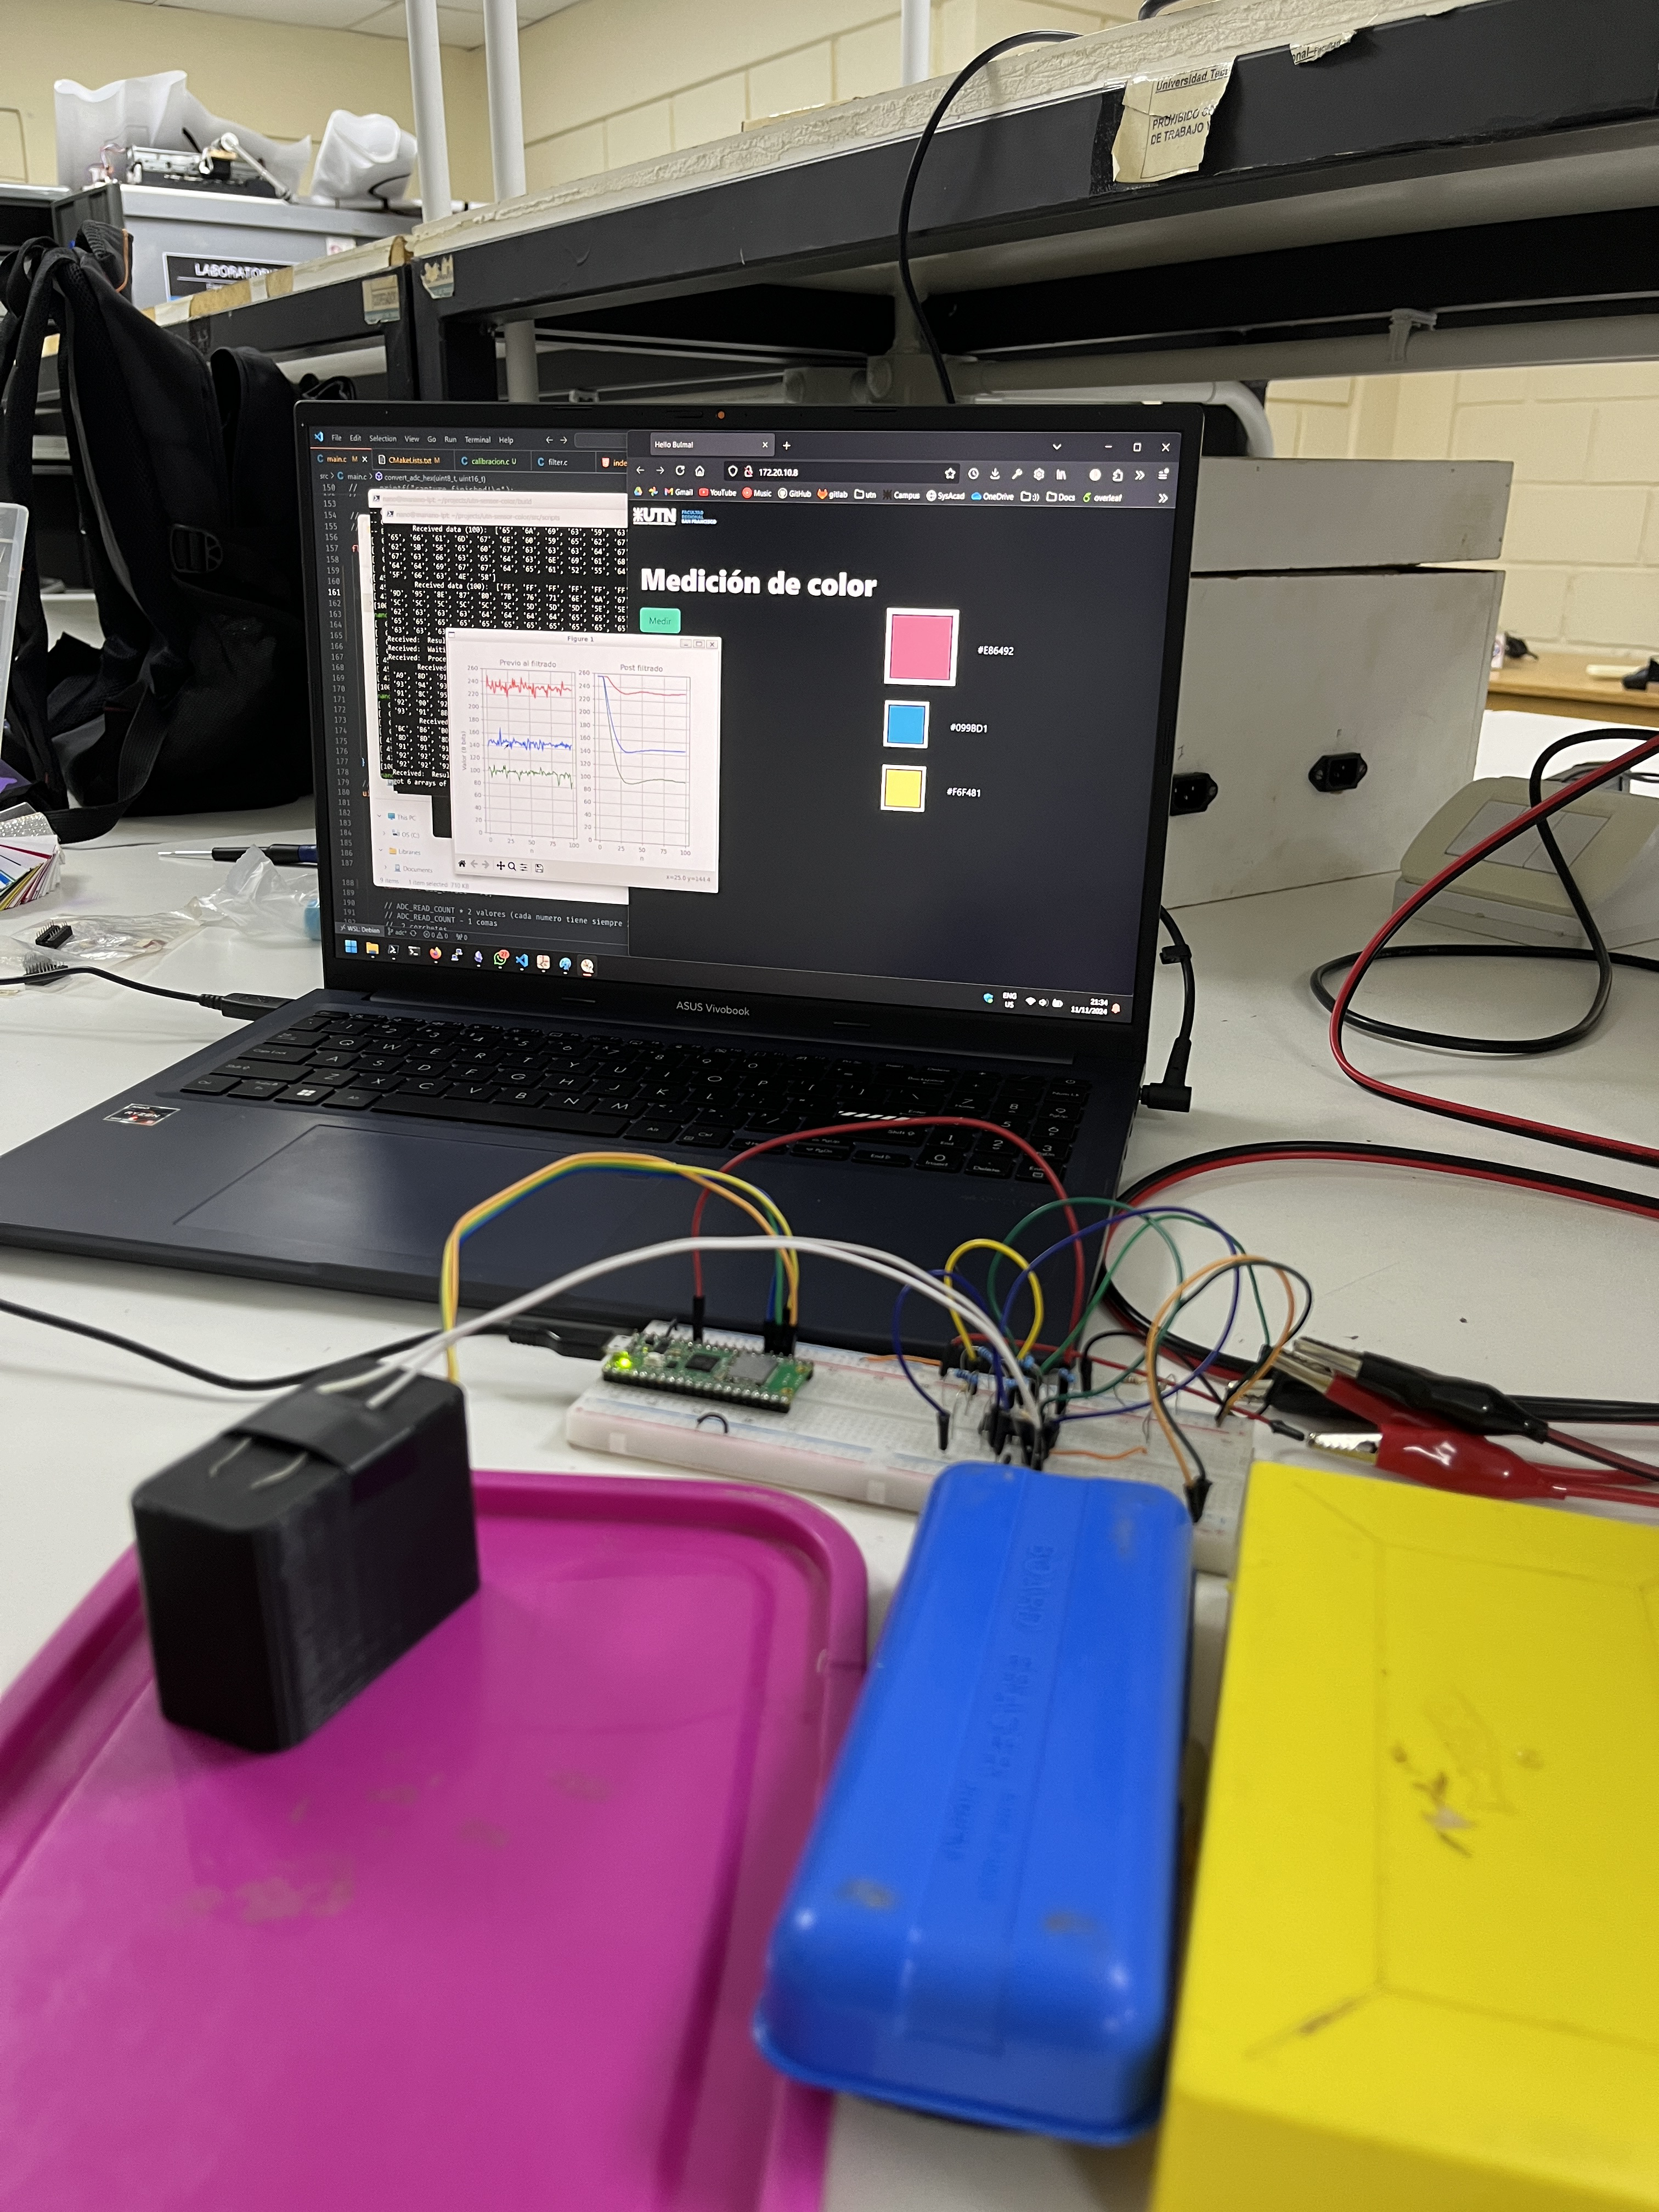
\includegraphics[width=0.8\linewidth]{img/resultados_sensor.png}
    \caption{Mediciones del sensor.}
    \label{fig:resultados}
\end{figure}
\end{document}


